\title{Упражнения за курса \\ Математически основи на машинното самообучение}

\author{}
%\author{Илия Мардов\thanks{
%		College of self-learning}
%	\and
%	DP\thanks{
%		The Virtual University
%	}\thanks{This work was
%		supported by NSB grant number G983578765401.}
%}

\documentclass{article}
\usepackage{amsmath}
\newtheorem{exercise}[subsubsection]{Упажнение}
\usepackage{graphicx}
\graphicspath{ {./images/} }
\usepackage{enumitem}

\usepackage{csquotes}[style=fallback]
\usepackage[T2A,T1]{fontenc}
\usepackage[main=bulgarian, english]{babel}

\usepackage[backend=biber]{biblatex} % 
\addbibresource{References.bib}
\usepackage{hyperref}

\usepackage{graphicx}
%\usepackage{listings}

\newtheorem{theorem}{Theorem}
\newtheorem{lemma}{Lemma}
\newtheorem{proposition}{Proposition}
\newtheorem{scolium}{Scolium}   %% And a not so common one.
\newtheorem{definition}{Дефиниция}

\usepackage{amssymb} % for blackbox
\newenvironment{proof}{{\sc доказателство:}}{~\hfill $\blacksquare$ }
\newenvironment{AMS}{}{}
\newenvironment{keywords}{}{}
%%%%%%%%%%%%%%%%%%%%%%%%%%%%%%%%%%%%%%%%%%%%%%%%%%%%%%%
\usepackage{pythonhighlight}

\begin{document}
	\newpage
	\date{}
	\maketitle

	\begin{abstract}
		Упражнения за курса Математически основи на машинното самообучение
	\end{abstract}
	
	\tableofcontents
		

	% \section*{0  \hspace{0.4cm}Упражнение 0. Python, R, инсталиране на среда}

\section{Уводни бележки. Базов Python. Линейна регресия.}
	\subsection{Уводни бележки}
	Мотивация - Курсът има широко приложение в индустрията.\\	
	Литература:
	\begin{enumerate}
	\item  Introduction to statistical learning \cite{james2023introduction}.
	\item  Elements of Statistical learning  \cite{hastie01statisticallearning}.
	\end{enumerate}
	
	\noindent
	Какво ще съдържа курса? Приблизително съдържанието на тези записки. \\
	
	\noindent
	Исторически бележки - Vapnik theory.(може да се добавят няколко изречения) \\

	\noindent	
	Среда за писане на код - VsCode и/или Anaconda + Spyder, Jupyter Notebook. \\
 	Забележка: преди 2 години Anaconda стана платена при enterprise, имайте го предвид.\\
 	Тук ще изпозлваме Python 3.10.11, последната версия с prebuild инсталационен пакет от python.org,
 	от версиите 3.10.11. За 3.11 и наскоро излязлата 3.12 нямаме още всички пакети. Ако ще изпозлваме виртуална среда: 	
 	\begin{lstlisting}[language=bash]
$pip install virtualenv
 	\end{lstlisting}
 	(Да се добавят git clone и прочие... команди и и описания) \\
 	
 	Отваряме с VSCode папката с кода на упражненията и пишем:
	\begin{lstlisting}[language=bash]
$pip install -r requirements.txt
 	\end{lstlisting}
 	За инсталиране на пакетите, които се използват в курса. \\
 	Линк към страницата с Lab упражненията от книгата:\\
 	\href{https://intro-stat-learning.github.io/ISLP/installation.html}{https://intro-stat-learning.github.io/ISLP/installation.html}
 	
 	\subsection{Базов Python}
 	Най-базови неща в Python - python list, set, import packages, най-базови фунцкии в numpy,
 	събиране на вектори и умножение на вектори с число, скаларно произведение, матрици.
 	pandas пакета и пример за графика с matplotlib.pyplot.\\
 	
 	Lab 2.3 Introduction to Python от Python книгата. Линк: \\

 	\href{https://intro-stat-learning.github.io/ISLP/labs/Ch02-statlearn-lab.html#}{https://intro-stat-learning.github.io/ISLP/labs/Ch02-statlearn-lab.html\#}.
 	
	\subsection{Линейна регресия}
	Данни, разглеждане - упражнение 2.8, 2.9 или 2.10 от Applied. \\
	(!) Добре е или да се разгледат функциите load\_data() от ISLP пакета или
	да се изнесе частта от кода за конкретния dataset при упражненията.
	
	Преговаряне на метод на най-малките квадрати: \\
	Нека имаме множество от точки $(x_1,y_1), (x_n,y_n), \dots (x_n,y_n)$. 
	Права от вида $\hat y = \hat \beta_0 + \sum \hat \beta_i  x_i $, която минимизира $\sum (y-\hat{y})^2$  може да се намери с метод на най-малките квадрати. \\
	С какво е полезна линейната регресия? Mоже да се използва за $"$старт$"$.\\
	Плюсове и минуси - прост модел, лесно се смята и разбира, лесно се обяснява, недоба в нелинейни задачи. \\
	
	Да се добави Мultiple regression и значение на променливите, примерът на Hastie and Tibshirani с успоредни прави. \\
	
	Следва Lab 3.6 
	\subsection{Упражнения}
	В зависимост от отделеното време на въведение в Python,
	2 от 3 по-долу може би ще е добре
	
	\begin{exercise}[2.8]
		This exercise relates to the College data set, which can be found in
		the file College.csv on the book website. It contains a number of
		variables for 777 different universities and colleges in the US. The
		variables are
		\begin{itemize}
			\item $\mathbf{Private}$ : Public/private indicator
			\item Apps : Number of applications received
			\item Accept : Number of applicants accepted
			\item Enroll : Number of new students enrolled
			\item Top10perc : New students from top 10 \% of high school class
			\item Top25perc : New students from top 25 \% of high school class
			\item F.Undergrad : Number of full-time undergraduates
			\item P.Undergrad : Number of part-time undergraduates
			\item Outstate : Out-of-state tuition
			\item Room.Board : Room and board costs
			\item Books : Estimated book costs
			\item PhD : Percent of faculty with Ph.D.s
			\item  Terminal : Percent of faculty with terminal degree
			\item S.F.Ratio : Student/faculty ratio
			\item perc.alumni : Percent of alumni wh
			\item Expend : Instructional expenditure per student
			\item Grad.Rate : Graduation rate
		\end{itemize}
	 Before reading the data into Python, it can be viewed in Excel or a
	 text editor.
	\begin{enumerate}[label=(\alph*)]
		\item  Use the pd.read\_csv() function to read the data into Python. Call
		the loaded data college. Make sure that you have the directory
		set to the correct location for the data.
		\item Look at the data used in the notebook by creating and running
		a new cell with just the code college in it. You should notice
		that the first column is just the name of each university in a
		column named something like Unnamed: 0. We don’t really want
		pandas to treat this as data. However, it may be handy to have
		these names for later. Try the following commands and similarly
		look at the resulting data frames:
		\begin{python}[language=Python]
college2 = pd.read_csv('College.csv', index_col=0)
college3 = college.rename({'Unnamed: 0': 'College'},
													axis=1)
college3 = college3.set_index('College')
	\end{python}		
This has used the first column in the file as an index for the
data frame. This means that pandas has given each row a name
corresponding to the appropriate university. Now you should see
that the first data column is Private. Note that the names of
the colleges appear on the left of the table. We also introduced
a new python object above: a dictionary, which is specified by dictionary
(key, value) pairs. Keep your modified version of the data with
the following:
\begin{python}
	college = college3
\end{python}

		\item Use the describe() method of to produce a numerical summary
		of the variables in the data set.
		\item Use the pd.plotting.scatter\_matrix() function to produce a
		scatterplot matrix of the first columns [Top10perc, Apps, Enroll].
		Recall that you can reference a list C of columns of a data frame
		A using A[C].
		\item Use the boxplot() method of college to produce side-by-side
		boxplots of Outstate versus Private.
		\item Create a new qualitative variable, called Elite, by binning the
		Top10perc variable into two groups based on whether or not the
		proportion of students coming from the top 10% of their high
		school classes exceeds 50%.
		\begin{python}
college['Elite'] = pd.cut(college['Top10perc'],
[0,0.5,1],
labels=['No', 'Yes'])
		\end{python}
		\item Use the value\_counts() method of college['Elite'] to see how
		many elite universities there are. Finally, use the boxplot() method
		again to produce side-by-side boxplots of Outstate versus Elite.
		\item Use the plot.hist() method of college to produce some his-
		tograms with differing numbers of bins for a few of the quanti-
		tative variables. The command plt.subplots(2, 2) may be use-
		ful: it will divide the plot window into four regions so that four
		plots can be made simultaneously. By changing the arguments
		you can divide the screen up in other combinations.
		\item Continue exploring the data, and provide a brief summary of
		what you discover.		
	\end{enumerate}		
	\end{exercise}

\begin{exercise}[2.9]
	This exercise involves the Auto data set studied in the lab. Make sure
	that the missing values have been removed from the data.
	\begin{enumerate}[label=(\alph*)]
		\item Which of the predictors are quantitative, and which are quali-
		tative?
		\item  What is the range of each quantitative predictor? You can an-
		swer this using the min() and max() methods in numpy.
		\item What is the mean and standard deviation of each quantitative
		predictor?
		\item  Now remove the 10th through 85th observations. What is the
		range, mean, and standard deviation of each predictor in the
		subset of the data that remains?
		\item Using the full data set, investigate the predictors graphically,
		using scatterplots or other tools of your choice. Create some plots
		highlighting the relationships among the predictors. Comment
		on your findings.
		\item  Suppose that we wish to predict gas mileage (mpg) on the basis
		of the other variables. Do your plots suggest that any of the
		other variables might be useful in predicting mpg? Justify your
		answer.
		
	\end{enumerate}
\end{exercise}
	\begin{exercise}[2.10]
		This exercise involves the Boston housing data set.
		\begin{enumerate}[label=(\alph*)]
		\item To begin, load in the Boston data set, which is part of the ISLP
		library.
		\item How many rows are in this data set? How many columns? What
		do the rows and columns represent?
		\item Make some pairwise scatterplots of the predictors (columns) in
		this data set. Describe your findings.
		\item Are any of the predictors associated with per capita crime rate?
		If so, explain the relationship. 
		\item Do any of the suburbs of Boston appear to have particularly
		high crime rates? Tax rates? Pupil-teacher ratios? Comment on
		the range of each predictor.		 
		\item How many of the suburbs in this data set bound the Charles
		river?		 
		\item What is the median pupil-teacher ratio among the towns in this
		data set?		 
		\item Which suburb of Boston has lowest median value of owner-
		occupied homes? What are the values of the other predictors
		for that suburb, and how do those values compare to the overall
		ranges for those predictors? Comment on your findings.	 	 
		\item In this data set, how many of the suburbs average more than
		seven rooms per dwelling? More than eight rooms per dwelling?
		Comment on the suburbs that average more than eight rooms
		per dwelling.
		\end{enumerate}
	\end{exercise}
	
		
		
		
\newpage	
\section{Логистична регресия. Linear Discriminant \\ analysis.}




	\subsection{Кратка информация}
	Мотивация - логистичната регресия се използва за Credit Score модели.\\
	Моделът има вида: \\
	$\mathbb{E}(Y|X_1, \dots, X_p) = Prob(Y=1|X_1, \dots, X_p) = \frac{e^{\beta_0 + \beta_1 X_1 + \dots + \beta_p X_p}}{1+ e^{\beta_0 + \beta_1 X_1 + \dots + \beta_p X_p}} $ \\
	$\mathbb{E}(Y|X_1, \dots, X_p) = Prob(Y=0|X_1, \dots, X_p) = \frac{e^{\beta_0 + \beta_1 X_1 + \dots + \beta_p X_p}}{1+ e^{\beta_0 + \beta_1 X_1 + \dots + \beta_p X_p}} $
	
	Идея за други класификационни модели - Linear Discriminant Analysis, Quadratic Discriminant Analysis, Naive Bayes.
	Naive Bayes - .... \\
	Linear Discriminant analysis \\
	Ако класовете са с многомерно гаусово разпределение, или
	$$f_k(x) = \frac{1}{(2\pi)^p/2 \left | \Sigma_k  \right |} e^{-\frac{1}{2} (x-\mu_k)^T \Sigma_k^{-1}(x-\mu_k)} $$
	в специалния случай, където ковариационните матрици са равни, $\Sigma_k = \Sigma \forall k$, имаме 
	Линеен дискриминантен анализ.
	
	Теорема на Bayes с доказателство(припомняне): 
	\begin{theorem}[Bayes]
		$P(A|B) = \frac{P(B|A)P(B)}{P(A)}.$
	\end{theorem}
	\begin{proof}
		По дефиниция $P(A|B) = P(A\cap B)P(B)$ и $P(B|A) = P(B\cap A)P(A)$. Получаваме
	 $P(A\cap B)= \frac{P(A|B) }{P(B)} = \frac{P(B|A) }{P(A)}$, откъдето следва равенството.
	\end{proof}

	
	\subsection{Упражнения}
	Conceptual 4.8 section, ex 1, 2, 12 \\

	\begin{exercise}[Sec 4.8, Conceptual ex. 1]
			Using a little bit of algebra, prove that (4.2) is equivalent to (4.3). In
		other words, the logistic function representation and logit represen-
		tation for the logistic regression model are equivalent.
	\end{exercise}

	\begin{exercise}[Sec 4.8, Conceptual ex. 2]
		А
	\end{exercise}


	\begin{exercise}[Sec 4.8, Conceptual ex. 12]
	Suppose that you wish to classify an observation $x \in R $ into apples
	and oranges. You fit a logistic regression model and find that
	
	Pr(Y = orange|X = x) =
	%exp(ˆβ0 + ˆβ1x)
	%1 + exp(ˆβ0 + ˆβ1x)
	.
	Your friend fits a logistic regression model to the same data using the
	softmax formulation in (4.13), and finds that
	$$Pr(Y= orange| X=x) = \frac{exp(\hat{a}_{orange} + \hat{a}_{orangex}) }{den}$$
	Pr(Y = orange|X = x) =
	%exp(ˆαorange0 + ˆαorange1x)
	%exp(ˆαorange0 + ˆαorange1x) + exp(ˆαapple0 + ˆαapple1x).
	(a) What is the log odds of orange versus apple in your model?
	(b) What is the log odds of orange versus apple in your friend’s
	model?
	(c) Suppose that in your model, $\beta_0$ and $\beta_1$. What are
	the coefficient estimates in your friend’s model? Be as specific
	as possible.
	(d) Now suppose that you and your friend fit the same two models
	on a different data set. This time, your friend gets the coefficient
	%estimates ˆαorange0 = 1.2, ˆαorange1 = −2, ˆαorange0 = 3, ˆαorange1 =
	0.6. What are the coefficient estimates in your model?
	(e) Finally, suppose you apply both models from (d) to a data set
	with 2,000 test observations. What fraction of the time do you
	expect the predicted class labels from your model to agree with
	those from your friend’s model? Explain your answer. \\
	\end{exercise}


	
	
	
	\newpage
	\section{Feature Selection. Model Selection - AIC, BIC. Bias-Variance tradeoff. K-fold Cross Validation.} 
	Weight of evidence, information value - използват се в индустрията, например при разработка на credit score модел, логистична регресия. \\
	В книгата има 4 подхода при избор на оптимален модел: \\
	$C_p$ статистика: $C_p = \frac{1}{n}(RSS + 2d \hat \sigma^2)$ за squared error loss
	\begin{itemize}
		\item $AIC = \frac{1}{n}(RSS + 2d \hat \sigma^2)$
		\item $BIC = \frac{1}{n}(RSS + log(n) d \hat \sigma^2)$
		\item $Adjusted \hspace{0.1cm} R^2 = 1 - \frac{RSS/(n-d-1)}{TSS/(n-1)} $
	\end{itemize}
	(да се добави значението на параметрите по-късно) \\
	(код за пресмятане с пример) \\
	
%	\begin{python}[language=Python]
%	def BIC_calc(free_param, stat, dof):
%	n = dof + free_param
%	k = free_param
%	return stat + np.log(n)*k
%\end{python}

	lab 6 за model selection \\
	Forward, Backward selection example \\
	Следните алгоритми са взети от книгата: \\
	Алгоритъм за best subset selection: 
	\begin{enumerate}
		\item Let M0 denote the null model, which contains no predictors. This
		model simply predicts the sample mean for each observation.
		\item For k = 1, 2, . . . p: 
			\begin{enumerate}
				\item Fit all $(?)$ p choose k models that contain exactly k predictors.
				\item Pick the best among these  $(?)$ p choose k models, and call it Mk. Here best
				is defined as having the smallest RSS, or equivalently largest R2.
			\end{enumerate}
		\item Select a single best model from among M0, . . . , Mp using using the
		prediction error on a validation set, Cp (AIC), BIC, or adjusted R2.
		Or use the cross-validation method
	\end{enumerate}
	
	Алгоритъм за Forward selection: 
	\begin{enumerate}
				\item Let M0 denote the null model, which contains no predictors.
		\item For k = 1, 2, . . . p: 
		\begin{enumerate}
			\item Consider all $p-k$   models that augment the predictors in Mk
			with one additional predictor.
			\item Choose the best among these$p-k$    models, and call it Mk+1.
			Here best is defined as having smallest RSS or highest R2.
		\end{enumerate}
		\item Select a single best model from among M0, . . . , Mp using the pre-
		diction error on a validation set, Cp (AIC), BIC, or adjusted R2. Or
		use the cross-validation method.
	\end{enumerate}
	
	
	Credit data\\
	
	5.3 Lab python book: Cross-Validation and the Bootstrap \\
	
\newpage
\section{Generalized linear models. Lasso, Ridge. Generalized additive models. }
\subsection{Generalized linear models}


	Lasso and Ridge from the book.\\
	Lasso formula, Ridge formula, explanation \\
	Въпрос: Как Ridge и Lasso fit-ват в общите линейни модели или
	общите адитивни модели?
	
	
	
	Да припомним няколко регресии, които сме виждали:\\
	\begin{itemize}
		\item линейна - $\mathbb{E}(Y|X_1, \dots, X_p) = \beta_0 + \beta_1 X_1 + \dots + \beta_p X_p $
		\item логистична -  $ \mathbb{E}(Y|X_1, \dots, X_p) = \frac{e^{\beta_0 + \beta_1 X_1 + \dots + \beta_p X_p}}{1+ e^{\beta_0 + \beta_1 X_1 + \dots + \beta_p X_p}} $
		\item Поансонова -  $ \mathbb{E}(Y|X_1, \dots, X_p) = e^{\beta_0 + \beta_1 X_1 + \dots + \beta_p X_p} $
 	\end{itemize}
	
	Общият линеен модел изглежда по следния начин(където $\eta$ е $"$свързваща фунцкия$"$):\\
	$$\eta(\mathbb{E}(Y|X_1, \dots, X_p)) = \beta_0 + \beta_1 X_1 + \dots + \beta_p X_p $$
	
	lab 6 за ridge lasso \\
	Change $\lambda$ for Lasso example.
	
	
	
	Подробно разписване на оптимизационната задача. Идея за множество от бъдещите задачи
	се разглеждат като оптимизационни.
	
\newpage	
\section{Нелинейни модели. Piecewise polynomials. Сплайни(Splines). Общи адитивни модели}
Lab 7.8 python \\
ex 7.9 6,10,11 \\
\subsection{Общи адитивни модели(Generalized additive models)}
Това е 7.7 от Python книгата. \\

Общ адитивен модел се за регресия се задава с уравненията(където заменяме $x_i$ с $f(x_i)$ от модела на линейна регресия):
$$y_i = \beta_0 + \sum_{j=1}^p f_j(x_{ij}) + \epsilon_i = \beta_0 + f_1(x_{i1}) + \dots + f_n(x_{ip}) + e_i $$
за $i = 0,1 \dots n$.
Общ адитивен модел се за класификация се задава с формулите:
$$ log(\frac{p(X)}{1-p(X)}) = \beta_0 + \beta_1 f_1(X_1) + \beta_2 f_2(X_2) + \dots + \beta_p f_p(X_p),$$
където отново $"$сме заменили $X$-овете от логистичната регресия с $f(X)$-ове$"$:
$$ log(\frac{p(X)}{1-p(X)}) = \beta_0 + \beta_1 X_1 + \beta_2 X_2 + \dots + \beta_p X_p $$

	
\newpage	
\section{Decision trees. Random fores. Bagging, boosting.}
	
\newpage
\section{Support Vector Machines. Метод на опорните вектори.}	
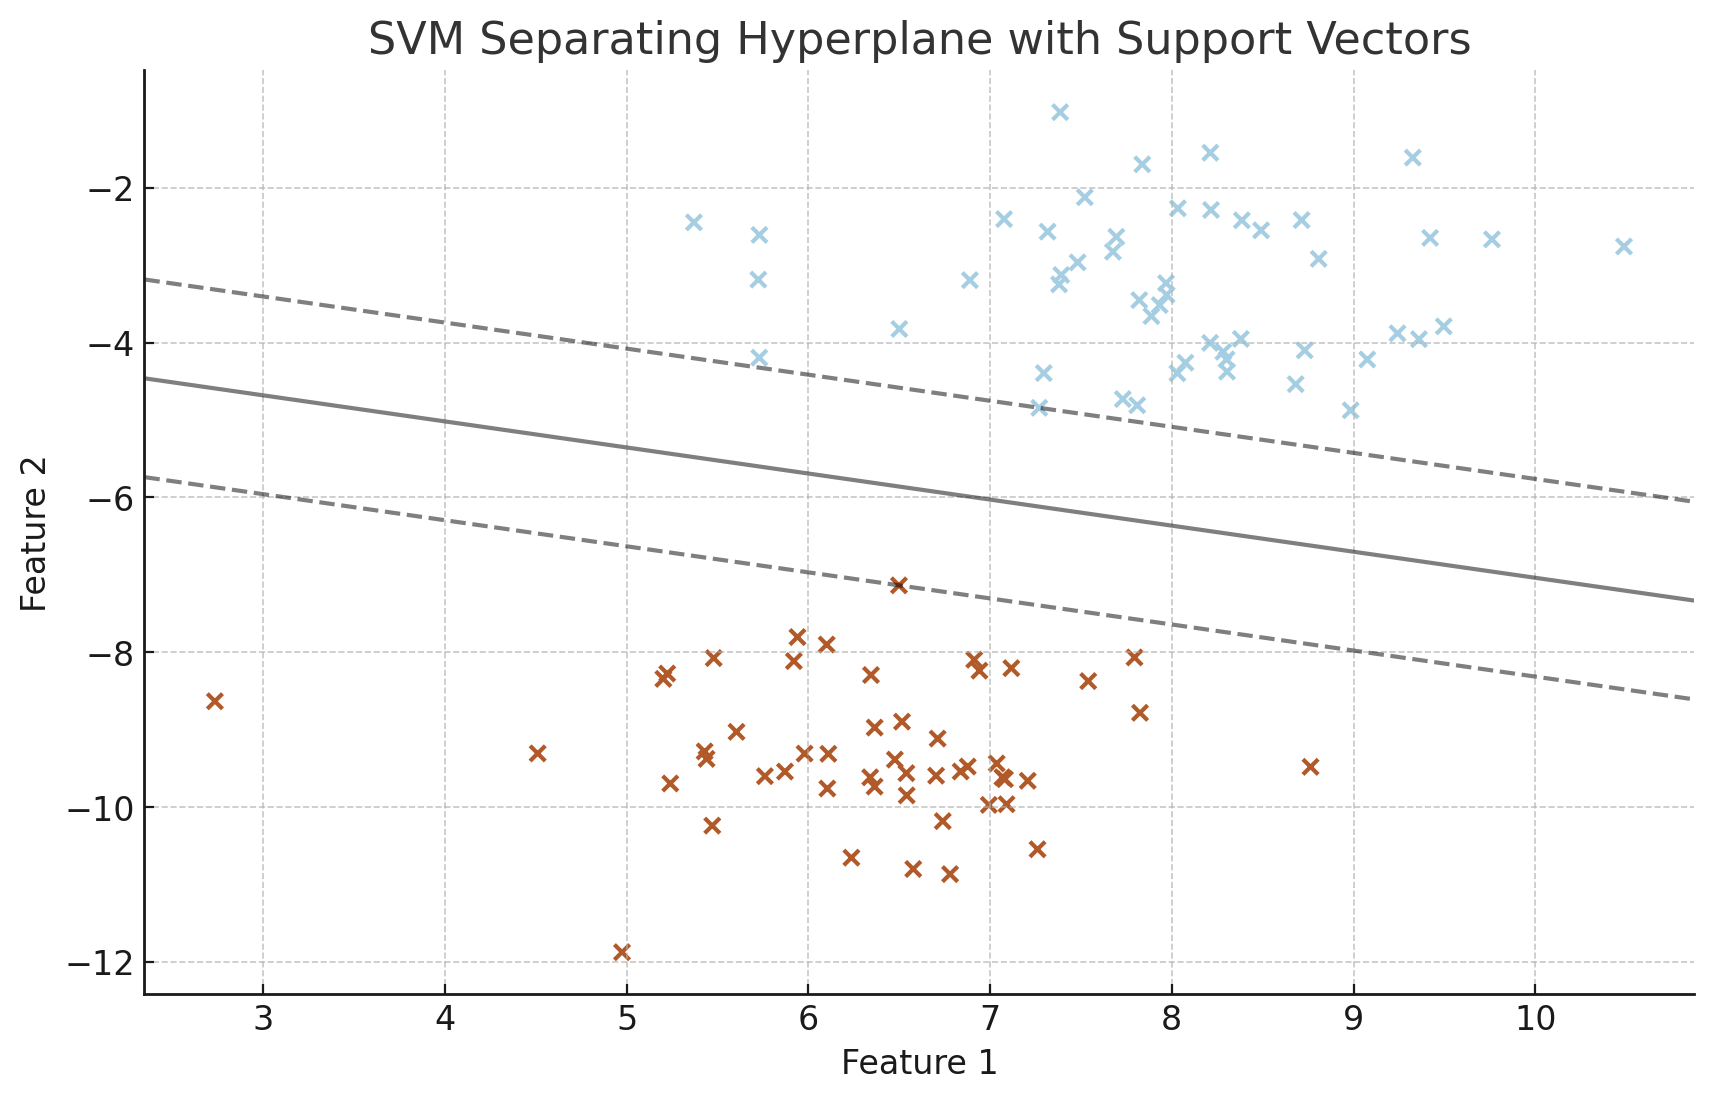
\includegraphics[scale=0.5]{svn.png}
Разделяща хиперравнина. \\
Recall: Хиперравнина се задава с $\beta_0 + \beta_1 X_1 + \dots + \beta_p X_p = 0$. Нормален вектор на тази хиперравнина
е $(\beta_1, \dots \beta_p)$ и той задава положителната посока. Уравнението може да се запише и като $\beta_0 + (\boldsymbol \beta, \mathbf X) = 0 $, където 
$\boldsymbol \beta = (\beta_1, \dots \beta_p) $ и $\mathbf X = (X_1, \dots, X_p)$. Една хиперравнина разделя пространството на две части, една с $\beta_0 + (\boldsymbol \beta, \mathbf X) > 0 $, и една с $\beta_0 + (\boldsymbol \beta, \mathbf X) < 0 $. Ако имаме точки в пространството, които можем да разделим с хиперравнина, и дадем labels на тези точки $y_i = 1$ и $y_i=-1$, то 
$$y_i(\beta_0 + \beta_1 x_{i1} + \dots \beta_p x_{ip}) > 0 .$$
Оптимизационна задача:
\begin{align}
%\begin{equation}
&\text{да се максимизира } M \\ 
%\end{equation}
%\begin{equation}
&\text{така че } \sum_{j=1}^{p} \beta_j^2 = 1 \\
%\end{equation}
%\begin{equation}
&	y_i(\beta_0 + \beta_1 x_{i1} + \dots \beta_p x_{ip}) \geq M \text{ за } i=1,\dots,n
%\end{equation}
\end{align}
Втора оптимизационна задача(Support Vector Classifier):
\begin{align}
&\text{да се максимизира } M \\ 
&\text{така че } \sum_{j=1}^{p} \beta_j^2 = 1 \\
&	y_i(\beta_0 + \beta_1 x_{i1} + \dots \beta_p x_{ip}) \geq M(1-\epsilon_i) \text{ за } i=1,\dots,n \\
& \text{ и } \epsilon_i \geq 0, \sum_i e_i = C 
\end{align}

Support Vector Machines:\\
Решението на втора оптимизационна задача може да се запише във вида
 $$ f(x) = \beta_0 + \sum_{i=1}^n \alpha_i \langle x,x_i \rangle , $$
 и тогава на нас са ни достатъчни скаларните произведения $ \langle x_i,x'_j \rangle $ за всички $ \binom{n}{2} $ двойки $x_i,x'_j $, $i,j = 1, \dots,n $, за да пресметнем модела.	
Вместо 	$ \langle x_i,x'_j \rangle $, може да вземем произволна kernel фунцкия $ K( x_i,x'_j ) $. Примерът със скаларното произведение 
е с линейна фунцкия, но може и нелинейна. \\

Упражнения: Conceptual 1,3 
	
\newpage
\section{Clustering. K-means clustering. Higherarchical clustering, Йерархично клъстериране}	
	\subsection{Clustering. K-means clustering}
	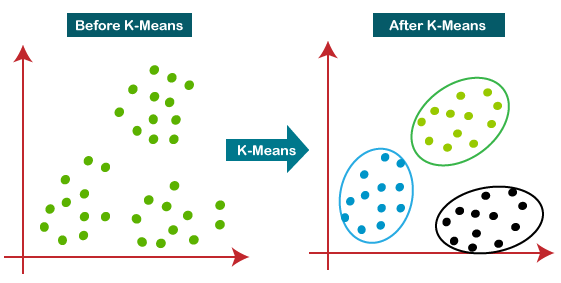
\includegraphics[scale=0.5]{k-means-clustering.png}
	\begin{definition}
		Клъстери на множеството $\{1, \dots, n\}$ наричаме подмножества $C_1 \cup \dots \cup C_K$, за които е изпълнено:
		\begin{enumerate}
			\item $C_1 \cup \dots \cup C_K = \{1, \dots, n\} ,$ 
			\item $C_i \cap C_j = \emptyset $ за всички $i \neq j.$
		\end{enumerate}
	\end{definition}

	Дефинираме оптимизационна задача:\\
	\begin{align}
	& \text{minimize} \Big\{ \sum_{j=i}^K W(C_i) \Big\} \\
		& W(C_i) = \frac{1}{C_i} \sum_{j,l \in C_i} \sum_{s=1}^p (x_{js}-x_{ls}) ^2
	\end{align}

	Алгоритъм за K-means: \\
	Algo \\
	\subsection{Higherarchical clustering}
	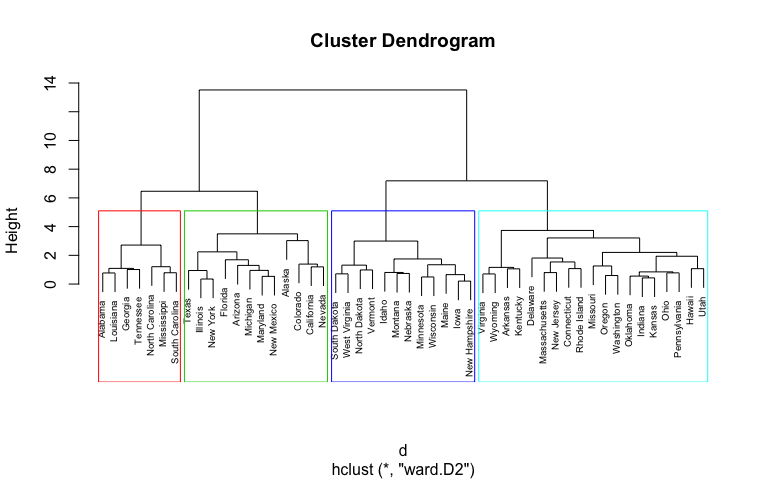
\includegraphics[scale=0.45]{hierarchical_clustering.png}


	Упражнения: \\
	K means ex 1 and 3, 10 \\
	Chapter 12, ex 13, hierarchical \\ 

	\cite{hastie01statisticallearning}
	
	
	\newpage
	
	\addcontentsline{toc}{section}{References}
	\printbibliography

%	\section*{About the author:}
%	We would like a short biographical sketch,
%	beyond just your affiliation to be placed
%	after the bibliography.
%	And below that, your full address.
%	
%	
%	
%	\subsection*{Primus Scriber}
%	College of the Enlightenment,
%	Philadelphia, Pennsylvania, 42345-6543$\pm\epsilon$.
%	pscriber@cenet.edu
%	
%	\subsection*{Theco Author}~
%	Department of Statistics,
%	The Virtual University,
%	New York, NY 13291-5555.
%	also@aol.com
	
\end{document}
